\subsection{Soluzioni implememtative per C++}
C++ è un linguaggio di programmazione molto complesso, ma anche molto versatile. Esso ben si presta 
ad implementare design pattern peculiari che in altri altri linguaggi non sarebbero possibili.

\subsubsection{Variant}
Il design pattern \textit{Variant} è un pattern che permette di implementare una union di tipi anche 
quando alcuni o tutti i tipi sono classi sono sprovvisti di un costruttore di default (senza argomenti).
In C++17 è stato introdotto il tipo \texttt{std::variant}, che permette di fare esattamente questo. All'interno 
della codebase di Basalt è possibile trovare una classe \texttt{SmartVariant} che è un wrapper su \texttt{std::variant}
e che espone una API più consona all'utilizzo specifico all'interno del progetto. \\

\subsubsection{Type-Erasure}
Il design pattern \textit{Type-Erasure} è un pattern che permette di avere vero e proprio polimorfismo 
object-oriented ma esponendo un API senza puntatori ed eventualmente ottimizzata con \textit{copy on write}.

\begin{figure}[H]
    \centering
        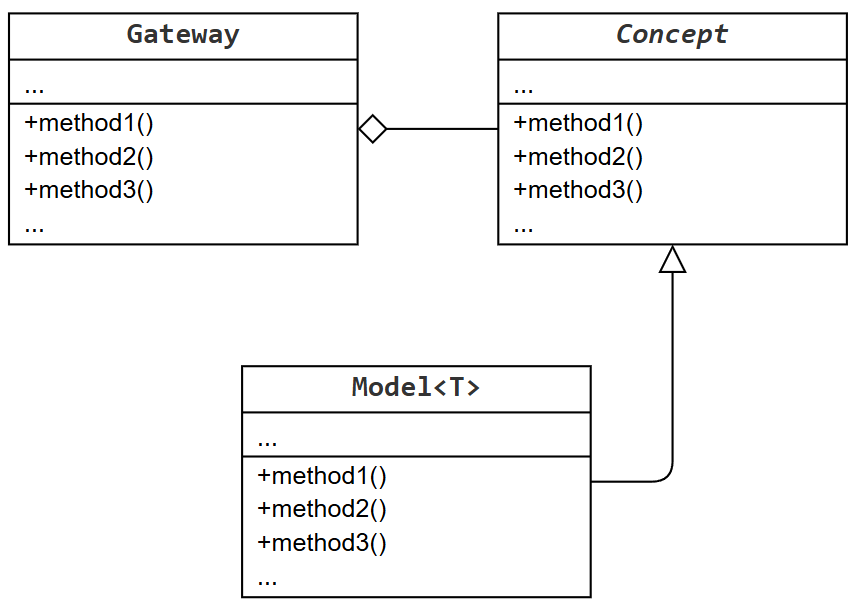
\includegraphics[width=0.7\textwidth]{../../Assets/TypeErasure.png}
    \caption{UML class diagram del pattern Type-Erasure}
\end{figure}

La classe \texttt{Gateway} è un esempio di implementazione di Type-Erasure. Essa viene utilizzata dai client 
come supertipo di tutti gli oggetti che implementano dei metodi pubblici chiamati \texttt{method1()}, 
\texttt{method2()},\texttt{method3()}, \texttt{method4()}, etc. \\

\newpage

Internamente essa possiede un puntatore ad \texttt{Concept}, a cui è possibile assegnare 
puntatori ad oggetti di tipo \texttt{Model<T>} per ogni scelta di \texttt{T}. \\

A patto che \texttt{T} esponga la corretta l'API, la classe \texttt{Model<T>} può implementare i metodi chiamandoli 
direttamente su di un'istanza di \texttt{T} che essa possiede come membro interno. \\

Assegnare un oggetto di tipo \texttt{T} ad un \texttt{Gateway} è possibile grazie alla ridefinizione dell'operatore \texttt{=}
nella classe \texttt{Gateway}. Assegnando un oggetto di tipo \texttt{T} a un oggetto di tipo \texttt{Gateway} allora 
il suo puntatore a \texttt{Concept} sarà aggiornato per puntare all'indirizzo di memoria di una cella appositamente allocata 
per contenere un \texttt{Model<T>} costruito a partire dall'oggetto \texttt{T} ricevuto. \\

\vspace{0.5cm}
\begin{lstlisting}[language=C++, frame=single]
#define ABSTRACT 0
template <typename T>
class Concept {
    public:
        virtual void method1() = ABSTRACT;
        virtual void method2() = ABSTRACT;
        //...
};

template <typename T>
class Model : public Concept {
    private:
        T object;
    public:
        Model(T obj) : object(obj) {}
        void method1() override { object.method1(); }
        void method2() override { object.method2(); }
        //...
};

class Gateway {
    private:
        std::unique_ptr<Concept> concept = nullptr;

    public:
        template<typename T>
        Gateway& operator=(T obj) {
            concept = std::make_unique<Model<T>>(obj);
        }

        void method1() { concept->method1(); }
        void method2() { concept->method2(); }
        //...
}

\end{lstlisting}
\vspace{0.5cm}

\newpage

questo pattern consente di assegnare a oggetti di tipo \texttt{Gateway} oggetti di tipo \texttt{T} che implementano
l'API corretta, e di chiamare i metodi di \texttt{T} attraverso l'oggetto di tipo \texttt{Gateway} senza 
usare esplicitamente puntatori, dereferenziazioni e senza dover deallocare manualmente nulla. \\

\subsubsection{Polymorph}
Il design pattern \textit{Polymorph} è un pattern creato specificamente per le esigenze della codebase di Basalt. Esso 
è derivante dal pattern Type-Erasure, ma con alcune sostanziali differenze. \\

\begin{figure}[H]
    \centering
        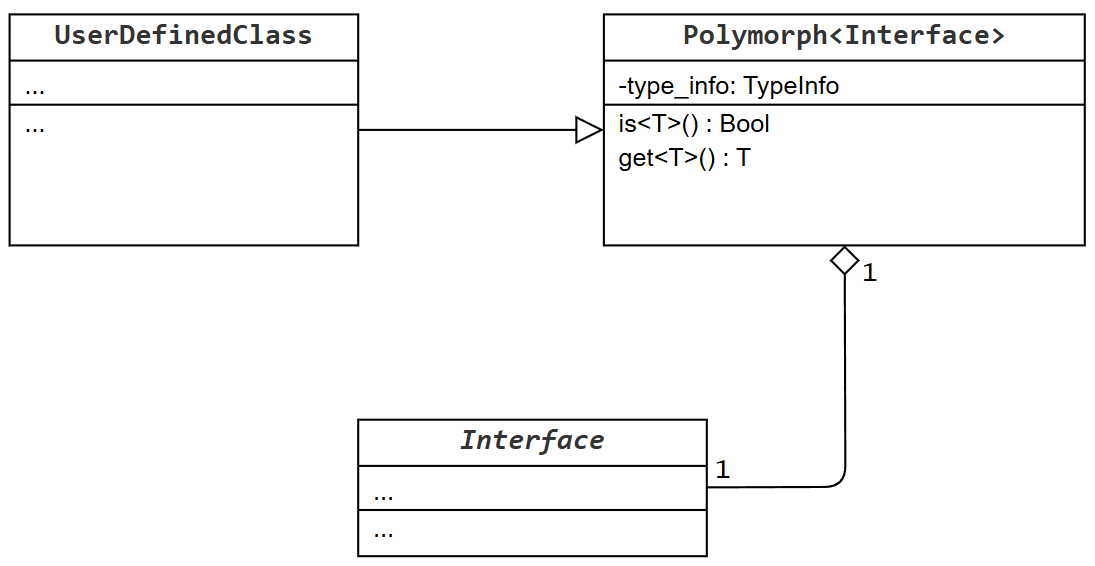
\includegraphics[width=0.7\textwidth]{../../Assets/Polymorph.png}
    \caption{UML class diagram del pattern Polymporph}
\end{figure}

Ogni classe definita dal client (ad esempio \texttt{UserDefinedClass}) deve estendere la classe \texttt{Polymorph<Interface>}. 
Facendo così, essa erediterà i metodi concreti \texttt{is} e \texttt{get} che permettono di fare \textit{downcasting}
dell'oggetto a runtime. \\

Contemporaneamente, sarà possibile assegnare a oggetti di tipo \texttt{UserDefinedClass} oggetti di tipo \texttt{T} purchè 
\texttt{T} estenda la classe \texttt{Interface} mediante ereditarietà. \\

Assegnando un oggetto di tipo \texttt{T} a un oggetto di tipo \texttt{UserDefinedClass} allora, essa utilizzerà l'operatore 
di assegnazione definito in \texttt{Polymorph} per assegnare ad un puntatore ad \texttt{Interface} l'oggetto che si desidera assegnare
ed aggiornare delle variabili interne per mantenere traccia del tipo dell'oggetto assegnato. \\

All'occorrenza si potrà interrogare la classe \texttt{UserDefinedClass} per sapere se contiene un oggetto di tipo \texttt{T}
o meno, utilizzando il metodo \texttt{is} e fare il \textit{downcasting} dell'oggetto a runtime utilizzando il metodo \texttt{get}. \\

\newpage

Di seguito è riportato un esempio di implementazione del pattern \textit{Polymorph}, così come è stato appena descrtto,
al netto della classe \texttt{UserDefinedClass}: \\

\vspace{0.5cm}
\begin{lstlisting}[language=C++, frame=single]
class Interface {
    public:
        //...
};

template <typename Interface>
class Polymorph {
    private:
        std::shared_ptr<Concept> ptr = nullptr;
        TypeInfo type_info;

    public:
        template <typename Implementation>
        Polymorph& operator=(Implementation obj) {
            ptr = std::make_shared<Interface>(obj);
            type_info = TypeInfo::from<Implementation>();
        }

        template <typename Implementation>
        bool is<>() 
            requires(std::is_base_of_v<Interface, Implementation>)
        { 
            return TypeInfo::from<Implementation>() 
                == type_info; 
        }

        template <typename Implementation>
        Implementation& get() 
            requires(std::is_base_of_v<Interface, Implementation>)
        {
            if (is<Implementation>()) {
                return *static_cast<Implementation*>(ptr.get());
            }
            throw std::runtime_error("Invalid downcast");
        }
}
\end{lstlisting}
\vspace{0.5cm}

\texttt{Interface} in questo caso serve solo ad essere estesa da tutte e sole le classi che si desidera 
assegnare al \texttt{Polymorph}. L'estendere \texttt{Interface} è necessario in quanto è stato 
introdotto tale vincolo usando \texttt{requires(std::is\_base\_of\_v<T,U>)} (C++20 concepts).

\newpage

\subsubsection{Notazioni e diagrammistica}
Dato che questi design pattern servono a rendere il codice più leggibile e mantenibile, astraendo rispetto 
a come un certo comportamento polimorfico sia stato implementato, non renderebbe giustiza alla codebase di Basalt 
l'essere rappresentata con un UML class diagram tradizionale, in quanto essa risulterebbe artificiosamente più complessa. Per 
questo motivo, si è deciso di utilizzare la notazione UML di sotto-tipo (is-a relationship) per rappresentare
non solo l'ereditarietà, ma anche l'implementazione di questi design pattern i quali rispecchiano proprio una 
relazione di sotto-tipo. \\

\begin{figure}[H]
    \begin{tikzpicture}
        \node (before) at(-1, 0) {
            \resizebox{9cm}{6cm}{   
                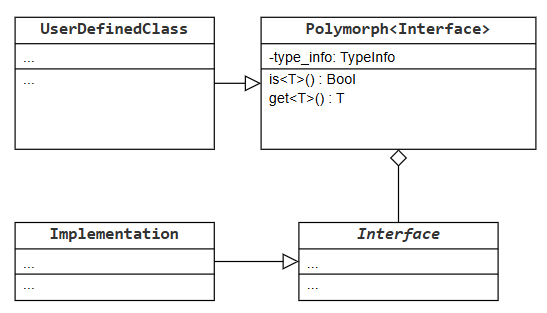
\includegraphics{../../Assets/Polymorph2.png}
            }
        };  

    
        \node[right of=before, xshift=7.5cm] (after) { 
            \resizebox{6cm}{8cm}{   
                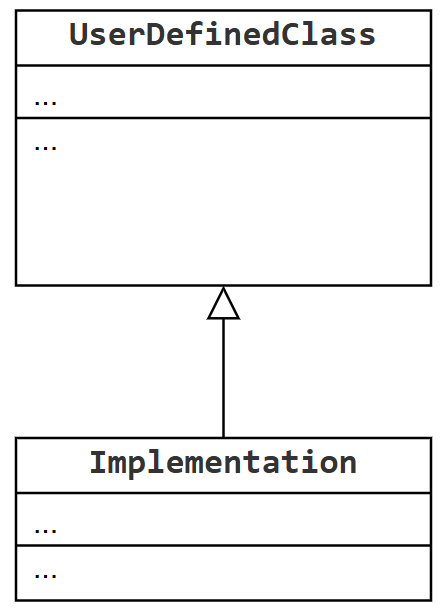
\includegraphics{../../Assets/Polymorph3.png}
            }
        };  

        \draw[->] (before) -- (after);
    \end{tikzpicture}
    \caption{
        \centering
        Traduzione UML del pattern Polymorph
    }
\end{figure}

\begin{figure}[H]
    \begin{tikzpicture}
        \node (before) {
            \resizebox{6.5cm}{6cm}{   
                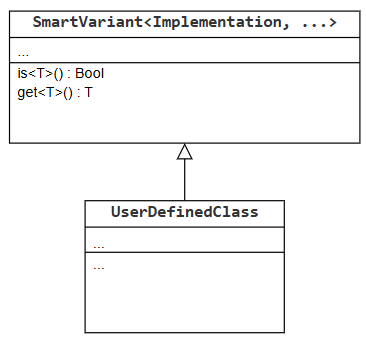
\includegraphics{../../Assets/SmartVariant.png}
            }
        };  

    
        \node[right of=before, xshift=7cm] (after) { 
            \resizebox{6cm}{8cm}{   
                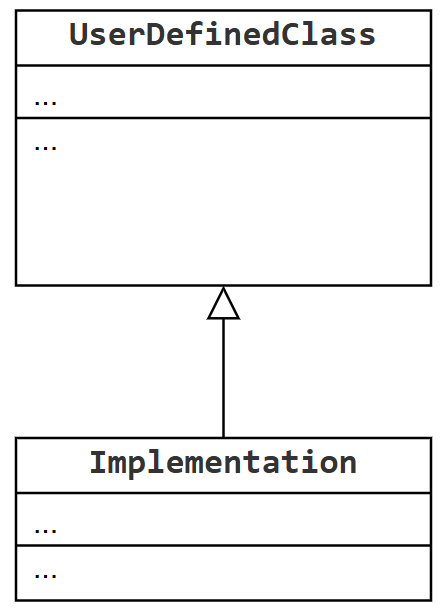
\includegraphics{../../Assets/Polymorph3.png}
            }
        };  

        \draw[->] (before) -- (after);
    \end{tikzpicture}
    \caption{
        \centering
        Traduzione UML del pattern Variant
    }
\end{figure}